% ---------------------------------------------------------------
% Section: BiLSTM Gap Filling
% ---------------------------------------------------------------

\section[BiLSTM Gap Filling]{BiLSTM Gap Filling vs Linear Interpolation}

\begin{frame}{BiLSTM Gap Filler --- Architecture}
\begin{columns}
\begin{column}{0.56\textwidth}
\textbf{Two-sided context encoders:}
\begin{itemize}\small
    \item Past LSTM over the pre-gap context
    \item Future LSTM over the post-gap context
    \item Each: hidden size 64, 2 layers, dropout 0.1
    \item Context length 10 frames on each side
\end{itemize}
\smallskip
\textbf{Per-step input (7 features):}
\begingroup\footnotesize
\begin{equation*}
    \left[x,\, y,\, \sin\varphi,\, \cos\varphi,\, \Delta x_{\rm prev},\, \Delta y_{\rm prev},\, \Delta t\right]
\end{equation*}
\endgroup
\textbf{Query inside the gap (3):}
\begingroup\footnotesize
\begin{equation*}
    \left[\alpha,\; \text{gap length},\; \text{offset}\right]
\end{equation*}
\endgroup
\end{column}
\begin{column}{0.44\textwidth}
\textbf{Fusion head (MLP):}
\begingroup\footnotesize
\begin{equation*}
    \big[\,h^{\rm past}_{-1} \oplus h^{\rm future}_{-1} \oplus q\,\big]
    \xrightarrow{\text{2$\times$ReLU}} \mathbb{R}^4
\end{equation*}
\endgroup
\textbf{Output = correction, not absolute:}
\begingroup\footnotesize
\begin{align*}
    (x,y) &= \text{linear interp.} + (\delta x, \delta y) \\
    \varphi &= \operatorname{atan2}(\sin\varphi, \cos\varphi)
\end{align*}
\endgroup
\begin{mynote}
\footnotesize Trained on artificial masked gaps from real consecutive detections (gap lengths 1, 2, 3, 5, 10). Measured rows are kept; the model only fills missing frames.
\end{mynote}
\end{column}
\end{columns}
\end{frame}

\begin{frame}{Masked-Gap Benchmark}
\begin{columns}
\begin{column}{0.64\textwidth}
\begin{figure}
    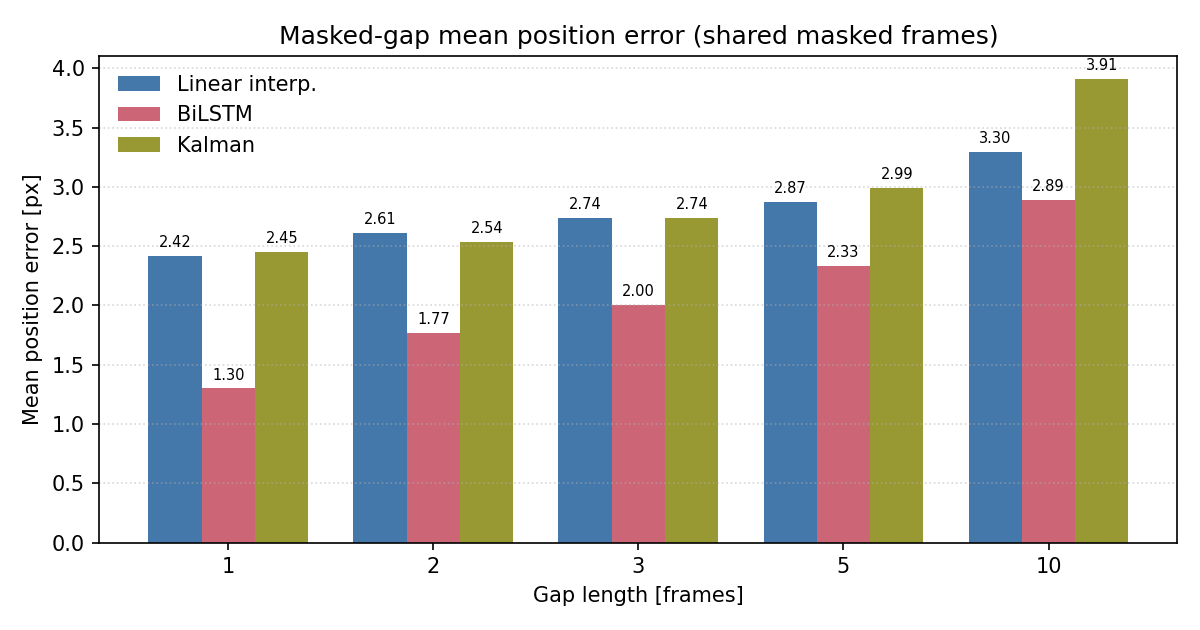
\includegraphics[width=\textwidth]{imglib/progress_update/bilstm_gap_benchmark.png}
\end{figure}
\end{column}
\begin{column}{0.36\textwidth}
\begin{myalert}[Result]
\small BiLSTM improves masked-gap error only because it uses both pre-gap and post-gap context.
\end{myalert}
\smallskip
\begin{mynote}
\footnotesize Mean error: BiLSTM 2.42 px, linear 2.99 px, Kalman 3.28 px.
\end{mynote}
\end{column}
\end{columns}
\end{frame}

\begin{frame}{Production Impact Is Small}
\begin{columns}
\begin{column}{0.58\textwidth}
\begin{figure}
    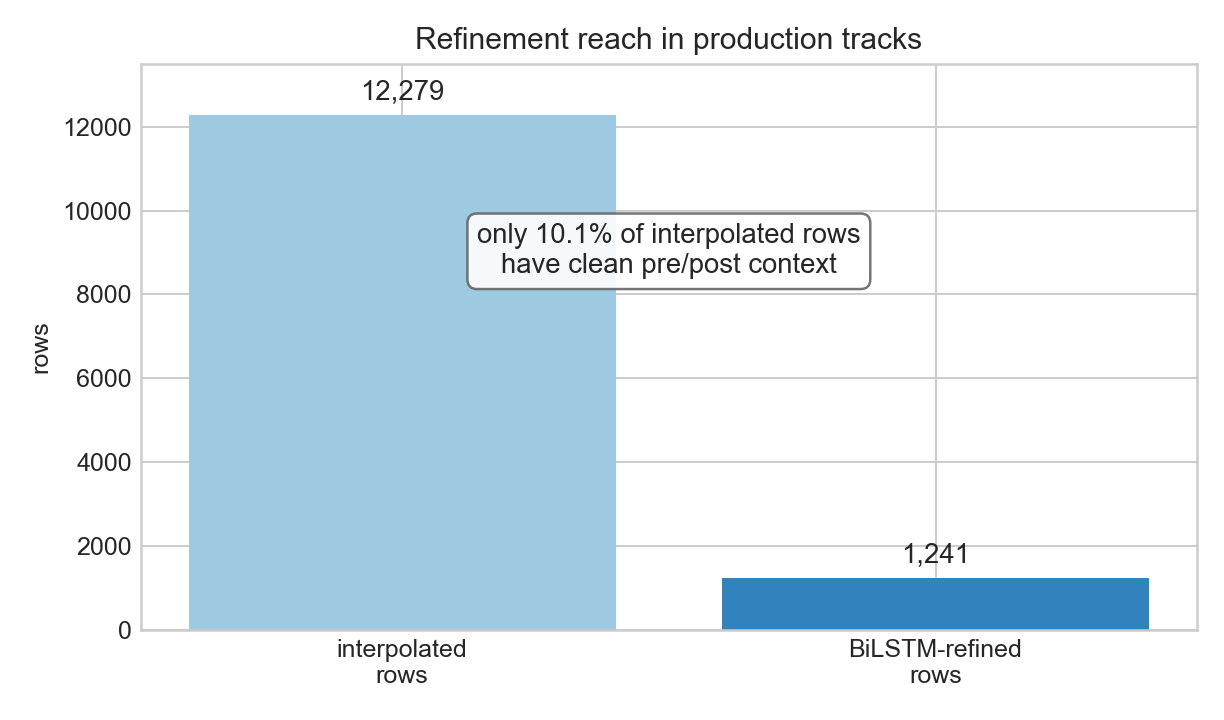
\includegraphics[width=\textwidth]{imglib/progress_update/bilstm_refinement_reach.png}
\end{figure}
\end{column}
\begin{column}{0.42\textwidth}
\begin{myalert}[Decision]
\small The main choice is whether interpolated rows should enter physics analysis, not which smoother fills them.
\end{myalert}
\smallskip
\begin{mynote}
\footnotesize ABP parameters for BiLSTM/Kalman-refined tracks stay close to the linear-interpolation variant.
\end{mynote}
\end{column}
\end{columns}
\end{frame}
